\section{Planen}


\subsection{Einführung}

\begin{frame}[c]{Pläne sind Nutzlos}
    \normalsize
    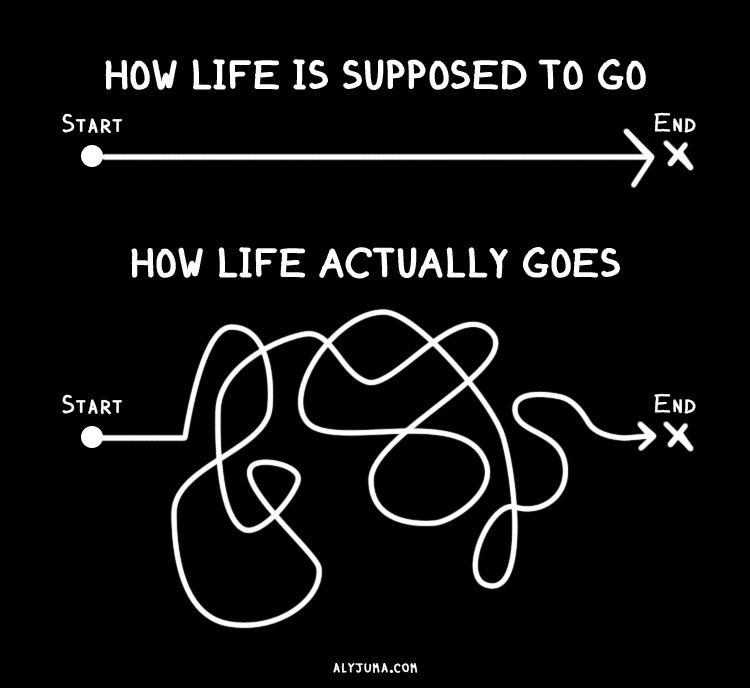
\includegraphics[height=0.9\textheight]{lifepath}
    Bild von \cite{lifepath-pic}
\end{frame}


\begin{frame}[c]{Planlosigkeit garantiert Scheitern}
    \begin{aquote}{Benjamin Franklin}
        If you fail to plan, you are planning to fail!
    \end{aquote}
\end{frame}

\begin{frame}[c]{Warum Planen}
    \large
    Man möchte Verstehen:
    \begin{itemize}[<+(1)->]
        % \item Versuch, das Ziel zu verstehen
        \item \textbf{Wann} das Ziel erfüllt ist
        \item \textbf{Was} der momentane Stand ist
        \item \textbf{Wie} das Ziel erreicht werden kann
        \item Welche \textbf{Hindernisse} auf dem Weg sind
        \item Was die \textbf{nächsten Schritte} sind
    \end{itemize}
    \pause
    Kurz: Die \textbf{Gesamtsituation}
\end{frame}


\subsection{Erfolg Definieren}
\pnote{Auf Ablauf eingehen}


\begin{frame}[c]{Problem: Ziel ist Unklar}
    \normalsize
    \includegraphics[width=\textwidth]{unclear-goals} \\
    How to wreck your finances. (Bild von \cite{unclear-goals-pic})
\end{frame}


\begin{frame}[c]% {Aufgabe: Klar definieren, wann das Ziel erreicht ist}
    % \begin{exampleblock}{Aufgabe}
    %     Definiere für jedes Ziel eindeutig, wann dieses Erreicht worden ist.
    % \end{exampleblock}
    % \begin{alertblock}{Aufgabe}
    %     Definiere für jedes Ziel eindeutig, wann dieses Erreicht worden ist.
    % \end{alertblock}
    \begin{block}{Aufgabe: Definiere Erfolg}
        Definiere für jedes deiner Ziele \textbf{eindeutig}, wann es erreicht wurde.
    \end{block}
    \pnote{Zeit: 5-10min}
\end{frame}

% We first need a clear-cut definition as to when the goal is achieved. You
% might have heard of ‘SMART’ goals before, Specific, Measurable, Achievable,
% Robust and Time-bound. I want you to focus on Specific and Measurable first,
% since they are good indicators of having achieved the goal. For each of your
% goals, be as specific as you realistically can about what you want. If
% possible, find something measurable.
%
% When trying to learn French, your Specific and Measurable goal might be to be
% capable of longer-duration interactions with native speakers, without a major
% stumble or needing to look up words; with the goal being achieved when you
% had five such 30min interactions. It does not need to be the full mastery of
% a language, ‘getting my driver’s license’ is a decent goal criterion for
% ‘learn to drive’.
%
% For all of your goals, clearly define when you have achieved them.
%
% Usually the best way is to ask how people who have achieved what you want to
% do knew that they have achieved it. You might want to do this later and adapt
% your own criteria based on their answers. While you’re at it, ask them about
% some tips for the way.


\subsection{Meilensteine}


\begin{frame}[c]{Problem: Abhängigkeiten}
    \normalsize
    
\includegraphics[height=0.9\textheight]{dependency}
    (Bild von \cite{dependency-pic})
\end{frame}



\begin{frame}[c]
    \begin{block}{Aufgabe: Definiere Meilensteine}
        Finde alle Meilensteine (\blue{Projekte}, nicht \green{Aufgaben}), die
        notwendig sind, um deine Ziele zu erreichen.
    \end{block}
    \pnote{Zeit: 5-10min}
\end{frame}


% Defining Sub-goals (5-10min)
% Bigger goals tend to have steps. They are not just done suddenly, there are
% steps in between that need to be achieved, sometimes in a specific order,
% before the actual goal can be achieved. When you want to do that awesome
% trip, you need to book the hotel beforehand, you need to check if you need to
% apply for visas, and buy new hiking shoes if you need some. These are all
% milestones, or sub-goals that are necessary to achieve the actual goal.
% Progress on one of them means progress towards your goal.
%
% While you can work independently on some (booking hotel and buying new gear),
% others, like checking if visas are required visas, might create additional
% milestones - getting the required visas.
%
% Sub-goals should be achievable within a few days at most. It’s okay if they
% only need a few minutes - as long as they are conceptually enclosed.
% (Sometimes there are sub-goals of sub-goals, that’s ok too!)
%
% Find and write down all relevant sub-goals for each of your bigger goals.


\subsection{Scheitern durch Erfolg}

\begin{frame}[c]{Problem: Gefühl von Fortschritt}
    \large
    \begin{aquote}{Charlie Munger, Berkshire Hathaway}
        Don’t just do something ... stand there
    \end{aquote}
    \normalsize
    Zu: Wie man nicht auf Aktienfluktuationen überreagiert.
    \pnote{Häufig fühlt es sich nur nach Fortschritt an}
\end{frame}


\begin{frame}[c]
    \vspace{1cm}
    \begin{block}{Aufgabe: Gefühlter Fortschritt}
        Versuche Situationen zu finden, die sich nach Fortschritt anfühlen
        könnten, aber nicht deinem Ziel näher kommen.
    \end{block}
    \vspace{0.5cm}
    \begin{block}{Aufgabe: Versuche zu Cheaten}
        Finde Möglichkeiten, den Weg zu deinem Ziel abzukürzen. Schreibe
        alles auf, was dir in den Sinn kommt. Nutze jede Abkürzung, die auch
        wirklich dein Ziel erreicht!
    \end{block}
    \pnote{Zeit: 15min}
    \pnote{Auch: Wie du dir selbst vorgaukeln könntest, es wäre Fortschritt ('es fühlt sich so an')}
\end{frame}


% Death by Winning (5min)
% Sometimes, it feels like we are working towards a goal and being successful,
% but we are actually not.
%
% There is a story of the early days of the X.com/PayPal rivalry. They were
% both frantically trying to put in more hours than the other and trying to get
% one more feature than the other. And for them it felt like progress. Except:
% It did not matter. Customers mostly ignored these features.
%
% If all you care about is to keep the ship’s nose pointed east, you won’t
% notice the ship sinking. Working for years on your career will only amount to
% so much if you realize that your (now broken) family would have been more
% important.
%
% There are situations in which we think everything is going fine, and we see
% progress happening towards a goal. Only to realize after weeks, months, or
% sometimes years, that while the ship’s nose was pointed east, the sails have
% never been set. The ship did not move forward - in fact, the waves slightly
% pushed it back.
%
% There would have been a simple way to avoid that - just the additional check
% that the sails are set. Just one small thing. If we just had made sure that
% the boat is actually moving, we could be much closer to our goal.
%
% By avoiding these kinds of situations, you can avoid wasting immense amounts
% of time, effort, and energy. Just staying clear of those will improve your
% effectiveness tremendously.
%
% Look for ways you might ‘cheat’ your goal, and write them down. If it is an
% actual shortcut, use it! If it will instead not get you closer to your actual
% goal, stay away from it.




\subsection{Leit- und Verzögerungsmaße}
% Leitmaß & Verzögerungsmaß


\begin{frame}[c]{Beispiel: Gewichtsreduktion}
    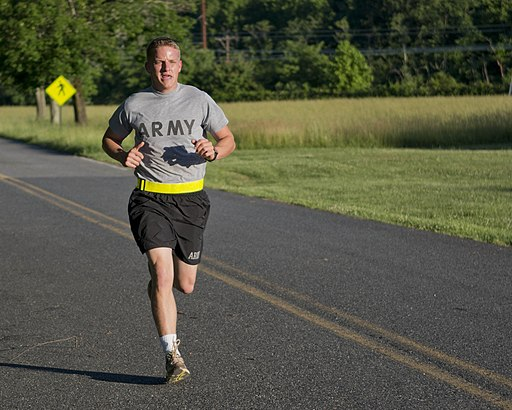
\includegraphics[height=0.8\textheight]{weight_loss} \\
    (Bild von \cite{weight-loss-pic})
    \pnote{Klassisches Neujahrsziel}
\end{frame}

\begin{frame}[c]{Definition: Verzögerungsmaß}
    \large
    \pause
    \textbf{Beispiel:} Gewicht
    \begin{itemize}[<+(1)->]
        \item Information über stand Jetzt oder Vergangenheit
        \item Was bereits passiert ist
        \item Einfach zu Erfassen
        \item Wird beeinflusst von vielen externen Faktoren
        \item Nützlich zu haben
        \item Aber kann nicht verändert werden
    \end{itemize}
    \pnote{Die meisten Wichtigen Dinge werden über Verzögerungsmaße gemessen}
    \pnote{Okay: Ziel Komplett erreicht (boolean)}
    \pnote{Muss nicht unbedingt 'graduell' sein}
\end{frame}


\begin{frame}[c]{Beispiel Gewicht: Einfluss Externer Faktoren}
    % trim = l b r t
    \small
    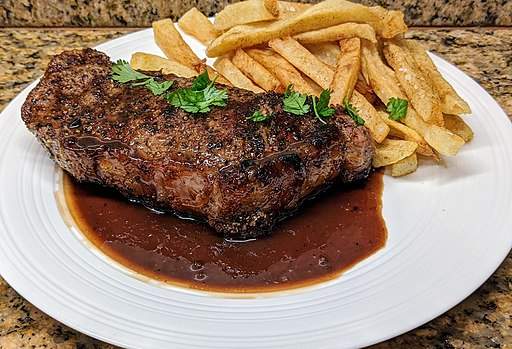
\includegraphics[width=0.7\textwidth, clip=true, trim = 15 150 15 20]{steak}
    (Bild von \cite{steak-pic})
    \large
    \begin{itemize}[<+(1)->]
        \item Getrunkenes Wasser
        \item Kohlenhydrate der letzten Tagen
        \item Verändert sich über den Tag
        \item Messung unter anderen Bedingungen
    \end{itemize}
\end{frame}

\begin{frame}[c]{Definition: Leitmaß}
    \large
    \pause
    \textbf{Beispiel:} Kaloriendefizit pro Tag
    \begin{itemize}[<+(1)->]
        \item Kann Erfolg Voraussagen
        \item Misst Aktionen, die Ergebnisse liefern
        \item Einfach zu Beeinflussen
        \item Häufig Schwer zu Messen
    \end{itemize}
    \pnote{Garantiert Ergebnisse}
    \pnote{Sollte graduell sein, muss es aber nicht}
    \pnote{Fokus sollte auf 'einfach messbar' sein}
\end{frame}


\begin{frame}[c]{Beispiel: Andrej Karpathy}
    \large
    Ziel: Defizit von ~500kcal pro Tag
    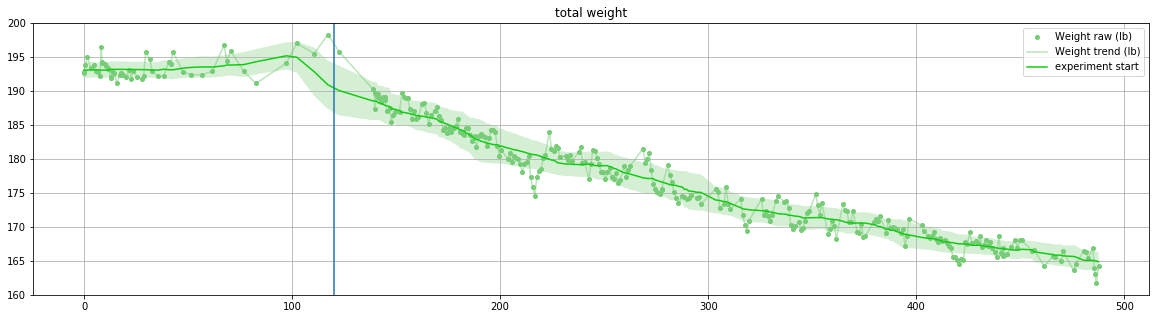
\includegraphics[width=\textwidth]{weight} \\
    (Bild von seinem Blog, \cite{weight-pic})
\end{frame}


% \begin{frame}[c]{Tipps für Leitmaße}
%     \large
%     \begin{itemize}[<+(1)->]
%         \item Bevorzuge robuste Maße (schwer zu Manipulieren)
%         \item Bevorzuge einfach Messbare Werte
%         \item Okay: Jeden Tag 30 minuten konzentriert Arbeiten
%     \end{itemize}
% \end{frame}


\begin{frame}[c]
    \begin{block}{Aufgabe: Definiere Leit- und Verzögerungsmaße}
        Versuche robuste Leit- und Verzögerungsmaße für jedes deiner Ziele zu
        Definieren.
    \end{block}
    \pnote{Zeit: 20min}
    \pnote{Verzögerungsmaß ist im zweifel einfach das Ziel selbst nach definierten Kriterien erreicht haben}
\end{frame}


% Exercises
% You get bonus points for robust Lead measures - if it’s hard for you to
% manipulate them, or cheat the measures in any way.
%
% For some goals (or even just some milestones) it is hard up to impossible to
% find good Lead measures - because circumstances, conditions and targets
% change so fast. You could meta-measure in these situations:
%
% Make one next action step towards the goal today, and make sure at least one
% is ready for tomorrow.
% I use similarly defined metrics for two of my goals.
%
% Go through your goals and Milestones and note which already have a Lag
% measure.
%
% Define Lead and Lag measures for each of your goals and milestones. If it
% seems impossible to find good Lead measures, set a timer to 3min and attempt
% to find one during this time.




% \begin{frame}[c]{Definition: Lag Measure}
%     \begin{itemize}[<+(1)->]
%         \item Information about the past
%         \item what already happened
%         \item easy to capture
%         \item It's useful to keep score
%         \item but it can't be changed
%     \end{itemize}
% \end{frame}
%
%
% \begin{frame}[c]{Definition: Lead Measure}
%     \begin{itemize}[<+(1)->]
%         \item Predict success
%         \item measure actions, that generate results
%         \item easy to influence
%         \item (sometimes) hard to capture
%     \end{itemize}
% \end{frame}


% We first take a good look at what Lead and Lag measures are before using them
% to make our goals and milestones more tangible.
%
% The fallacy of Lag measures
% A classical new-years goal is to lose weight. Let’s say the goal is to lose
% 10 kg until next year. At first, losing weight is rapid and easy. Until
% suddenly, you gain a bit. But then you lose weight again. And the reverse
% again. Your actual weight is fluctuating a lot, and it does not really feel
% like progress at all. This goes on for a bit, until most people quit.
%
% When trying to lose weight, weight is the thing you want to get down
% long-term. But there are a lot of factors influencing weight in the
% short-term. These include factors such as the time of day when measuring, how
% much water you just drank, the percentage of carbohydrates in last weeks’
% diet, and so much more. All of them can influence your weight right now
% tremendously. Noticing actual trends is hard, and impossible with less than
% two weeks of data. Most quit before a trend can manifest - but they couldn’t
% see a trend in the first place, since they don’t remember last week’s exact
% measure.
%
% Weight, just like most interesting metrics, is a Lag measure. While it is
% your ultimate goal, it is very susceptible to a wide range of factors and
% thus quite volatile in the short term. It is only useful in averages and
% long-term-trends. Results lag behind if you will. Looking at it today and
% feeling depressed about it will not do you any good - and it will not get you
% closer to your goal, either. So what if you want to measure something to feel
% good about it?
%
% Lead measures
% What you could measure instead, is daily calorie intake. Not just the intake,
% but ensuring that you have a certain calorie deficit each day. With a daily
% deficit of 500kcal, you are short 3500kcal every week, which is the energy
% stored in roughly 500g fat. The biggest benefit: it’s something that can be
% done every day, and it’s not susceptible to short-term variance. Keeping this
% up for Half a year will make you weigh less about 13.5 kg - a third more than
% the initial years’ goal of 10 kg.
%
% Daily calorie deficit is a Lead measure. Lead measures have much shorter
% intervals, such as days or weeks, and lead to the goal - eventually. For
% these, consistency is key. Consistently hitting your lead measures ensures
% that you hit your lag measures as well.
%
% Tips for applying them
% A Lag measures can be singular as well: ‘Finish writing the Goal Setting
% Workshop post’ is a current Lag measure for a milestone of mine. It does not
% necessarily have to be clear how lag measures are achieved, but it should be
% clear how to hit the lead measures.
%
% Lead measures might change across milestones, the important part is having a
% Lead measure for each milestone.
%
% It is absolutely okay for both Lead and Lag measures to be time-bound: One of
% my Lead measures is to read 30min in a focused manner each day. Sometimes I
% read up to two hours, but 30min is the minimum. No average, no ‘but I did
% double yesterday’, 30min a day, every day. This takes away the pressure to
% achieve a bit. This is especially useful when it is hard to estimate workload
% - I just cannot estimate the time required for reading a chapter or even a
%   single page, since both chapters and pages are sometimes more, and
%   sometimes less dense with information. Making it time-bound increases
%   predictability as well: you’re done after 30min, continue tomorrow - though
%   of course, there’s nothing stopping you from doing more work either, and
%   doing so feels incredibly good.
%
% Exercises
% You get bonus points for robust Lead measures - if it’s hard for you to
% manipulate them, or cheat the measures in any way.
%
% For some goals (or even just some milestones) it is hard up to impossible to
% find good Lead measures - because circumstances, conditions and targets
% change so fast. You could meta-measure in these situations:
%
% Make one next action step towards the goal today, and make sure at least one
% is ready for tomorrow.
% I use similarly defined metrics for two of my goals.
%
% Go through your goals and Milestones and note which already have a Lag
% measure.
%
% Define Lead and Lag measures for each of your goals and milestones. If it
% seems impossible to find good Lead measures, set a timer to 3min and attempt
% to find one during this time.


\subsection{Nächste Schritte}


\begin{frame}[c]{Problem: Ungewissheit}
    \large
    \begin{aquote}{Cassandra Clare}
        One must look at the next step on the path ahead, rather than the
        mountain in the distance, or one would never reach one's goal.
    \end{aquote}
\end{frame}


\begin{frame}[c]
    \begin{block}{Aufgabe: Finde die Nächsten Schritte}
        Finde die drei \green{Aufgaben} für jeden Meilenstein, die nicht lang
        dauern, und du direkt tun könntest. Erledige:
        \begin{itemize}
            \item die erste Aufgabe jetzt
            \item die zweite Aufgabe morgen vor 11 Uhr früh
            \item die dritte Aufgabe vor 11 Uhr früh übermorgen
        \end{itemize}
    \end{block}
    \pnote{Zeit: 10min}
\end{frame}


% Identify Next Actions (10min)
% At every point along the way, it is extremely important to have specific next
% actions. Sometimes the only things getting you closer to your goal are
% actions. Execution will focus on that more, but here is the basic idea: When
% in a situation where you could easily make progress towards your goals, you
% will not do so if you are unaware of the possibility.
%
% A next action is a clearly defined and described physical action that can be
% done immediately (if not blocked) and will bring you closer to one of your
% goals or milestones. Sometimes next actions are blocked, since you are
% waiting for a mail first, or need someone else to help you - be aware of
% those blockers.
%
% If you want to build an awesome tree house, and you go to the hardware store
% (getting color to paint a room), it can help to know if you need nails or
% not. If you noticed a week later, you would need more energy and momentum to
% go to the hardware store again. Knowing things like that at the right time
% will save a lot of energy and effort.
%
% Everything requiring more than two next actions to get it done is a project.
% Goals and milestones are necessarily projects, but you might be working on
% projects that are not part of your primary goals as well. Organizing a
% birthday party is unlikely part of your goals, but nonetheless something you
% might have committed to doing.
%
% For each of your milestones, find three next actions you could work on right
% now, each taking a few minutes at most.
%
% Do the first now (or later, but today)! Do the next tomorrow before 11am (or
% no later than 4h after waking up, whichever comes first), and the third the
% day after tomorrow before 11am. Ensure that you have new next actions to work
% towards by then.
%
% Take a break before continuing with Execution. Skip to conclusions if you
% have an execution system like gtd already.

\fpause
